% see http://info.semprag.org/basics for a full description of this template
\documentclass[cm,linguex]{glossa}

% possible options:
% [times] for Times font (default if no option is chosen)
% [cm] for Computer Modern font
% [lucida] for Lucida font (not freely available)
% [brill] open type font, freely downloadable for non-commercial use from http://www.brill.com/about/brill-fonts; requires xetex
% [charis] for CharisSIL font, freely downloadable from http://software.sil.org/charis/
% for the Brill an CharisSIL fonts, you have to use the XeLatex typesetting engine (not pdfLatex)
% for headings, tables, captions, etc., Fira Sans is used: https://www.fontsquirrel.com/fonts/fira-sans
% [biblatex] for using biblatex (the default is natbib, do not load the natbib package in this file, it is loaded automatically via the document class glossa.cls)
% [linguex] loads the linguex example package
% !! a note on the use of linguex: in glossed examples, the third line of the example (the translation) needs to be prefixed with \glt. This is to allow a first line with the name of the language and the source of the example. See example (2) in the text for an illustration.
% !! a note on the use of bibtex: for PhD dissertations to typeset correctly in the references list, the Address field needs to contain the city (for US cities in the format "Santa Cruz, CA")

%\addbibresource{sample.bib}
% the above line is for use with biblatex
% replace this by the name of your bib-file (extension .bib is required)
% comment out if you use natbib/bibtex

\let\B\relax %to resolve a conflict in the definition of these commands between xyling and xunicode (the latter called by fontspec, called by charis)
\let\T\relax
\usepackage{xyling} %for trees; the use of xyling with the CharisSIL font produces poor results in the branches. This problem does not arise with the packages qtree or forest.
\usepackage[linguistics]{forest} %for nice trees!
\usepackage{longtable}

\title[General Equilibrium]{Graphical Economics\\
Review}
% Optional short title inside square brackets, for the running headers.

% \author[Paul \& Vanden Wyngaerd]% short form of the author names for the running header. If no short author is given, no authors print in the headers.
% {%as many authors as you like, each separated by \AND.
%   \spauthor{Waltraud Paul\\
%   \institute{CNRS, CRLAO}\\
%   \small{105, Bd. Raspail, 75005 Paris\\
%   waltraud.paul@ehess.fr}
%   }
%   \AND
%   \spauthor{Guido Vanden Wyngaerd \\
%   \institute{KU Leuven}\\
%   \small{Warmoesberg 26, 1000 Brussel\\
%   guido.vandenwyngaerd@kuleuven.be}
%   }%
% }

\author[Carlos Lezama]{
    \spauthor{Carlos Enrique Lezama Jacinto\\
  \institute{\hfill\break
Instituto Tecnológico\\
Autónomo de México}\\
  \small{\hfill\break
clezamaj@itam.mx}
  }%
  }

\usepackage{natbib}


% tightlist command for lists without linebreak
\providecommand{\tightlist}{%
  \setlength{\itemsep}{0pt}\setlength{\parskip}{0pt}}





\usepackage{multirow, array}
\usepackage{amsmath, amsthm}

\setlength{\parskip}{\baselineskip}

\newcommand{\dnorm}{\mathcal{N}}
\newcommand{\dunif}{\mathcal{U}}
\newcommand{\ev}{\text{E}}
\newcommand{\iid}{\text{i.i.d.}}

\newtheoremstyle{defn}
{}                % Space above
{}                % Space below
{\mdseries}        % Theorem body font % (default is "\upshape")
{}                % Indent amount
{\bfseries\sffamily}       % Theorem head font % (default is \mdseries)
{.}               % Punctuation after theorem head % default: no punctuation
{ }               % Space after theorem head
{}                % Theorem head spec
\theoremstyle{defn}
\newtheorem{defn}{Definition}

\newtheoremstyle{axiom}
{}                % Space above
{}                % Space below
{\mdseries}        % Theorem body font % (default is "\upshape")
{}                % Indent amount
{\bfseries\sffamily}       % Theorem head font % (default is \mdseries)
{.}               % Punctuation after theorem head % default: no punctuation
{ }               % Space after theorem head
{}                % Theorem head spec
\theoremstyle{axiom}
\newtheorem{axiom}{A\!\!}

\newtheoremstyle{thm}
{}                % Space above
{}                % Space below
{\mdseries}        % Theorem body font % (default is "\upshape")
{}                % Indent amount
{\bfseries\sffamily}       % Theorem head font % (default is \mdseries)
{.}               % Punctuation after theorem head % default: no punctuation
{ }               % Space after theorem head
{}                % Theorem head spec
\theoremstyle{thm}
\newtheorem{thm}{Theorem}

\newtheoremstyle{lem}
{}                % Space above
{}                % Space below
{\mdseries}        % Theorem body font % (default is "\upshape")
{}                % Indent amount
{\bfseries\sffamily}       % Theorem head font % (default is \mdseries)
{.}               % Punctuation after theorem head % default: no punctuation
{ }               % Space after theorem head
{}                % Theorem head spec
\theoremstyle{lem}
\newtheorem{lem}[thm]{Lemma}

\newtheoremstyle{cor}
{}                % Space above
{}                % Space below
{\mdseries}        % Theorem body font % (default is "\upshape")
{}                % Indent amount
{\bfseries\sffamily}       % Theorem head font % (default is \mdseries)
{.}               % Punctuation after theorem head % default: no punctuation
{ }               % Space after theorem head
{}                % Theorem head spec
\theoremstyle{cor}
\newtheorem{cor}{Corollary}[thm]

\newtheoremstyle{prop}
{}                % Space above
{}                % Space below
{\mdseries}        % Theorem body font % (default is "\upshape")
{}                % Indent amount
{\bfseries\sffamily}       % Theorem head font % (default is \mdseries)
{.}               % Punctuation after theorem head % default: no punctuation
{ }               % Space after theorem head
{}                % Theorem head spec
\theoremstyle{prop}
\newtheorem{prop}{Proposition}

\newtheoremstyle{rmk}
{}                % Space above
{}                % Space below
{\itshape}        % Theorem body font % (default is "\upshape")
{}                % Indent amount
{\slshape\sffamily}       % Theorem head font % (default is \mdseries)
{.}               % Punctuation after theorem head % default: no punctuation
{ }               % Space after theorem head
{}                % Theorem head spec
\theoremstyle{rmk}
\newtheorem*{rmk}{Remark}







\begin{document}


\sffamily
\maketitle


\begin{keywords}
  general equilibrium, local markets, graph theory, computer science
\end{keywords}

\rmfamily

%  Body of the article
\maketitle
\thispagestyle{empty}

\hypertarget{lecture-notes}{%
\section{Lecture Notes}\label{lecture-notes}}

The following pages will summarize the work of \citet{KKO} without
assuming any prior knowledge other than that obtained during the General
Equilibrium course lectured in Fall 2022 by
\href{https://www.xinyang-wang.com}{Xinyang Wang}.\footnote{This may
  include, but is not limited to, general equilibrium, graph theory, and
  computer science.}

\hypertarget{graph-theory}{%
\subsection{Graph Theory}\label{graph-theory}}

\begin{defn}[Graph]
A \textbf{graph} is a tuple $G = (V,E)$ where $V$ is a (finite) set of \emph{vertices} (also called \emph{nodes}) and $E$ is a finite collection of \emph{edges}. The set $E$ contains elements from the union of the one and two element subsets of $V$. That is, each edge is either a one or two element subset of $V$. $E$ is a subset of $V^{(2)} = \left\{\{x, y\} : x, y \in V,\ x \neq y \right\}$.

\begin{figure}[H]
\centering
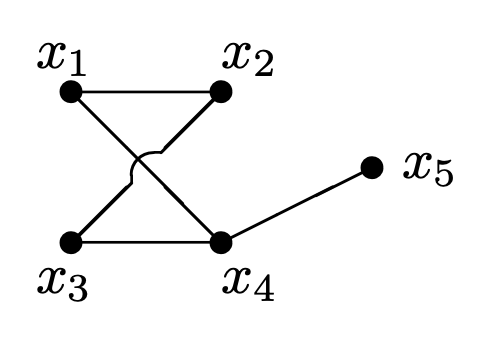
\includegraphics[scale=0.4]{fig/1.png}
\caption{$V = \{x_1, x_2, x_3, x_4, x_5\}$, $E = \{x_1 x_2, x_1 x_4, x_2 x_3, x_3 x_4, x_4 x_5\}$.}
\end{figure}
\end{defn}

\begin{rmk}
We call $V = V(G)$ the \textbf{vertex set} of $G$ and $E = E(G)$ the \textbf{edge set} of $G$.
\end{rmk}

\begin{defn}[Order]
The \textbf{order} of $G$ is $\lvert G \rvert = \lvert V(G) \rvert$.
\end{defn}

\begin{defn}[Size]
The \textbf{size} of $G$ is $e(G) = \lvert E(G) \rvert$.
\end{defn}

\begin{defn}[Self-Loop]
If $G = (V,E)$ is a graph, $v \in V$, and $e = \{v\}$, then edge $e$ is called a \textbf{self-loop}. That is, any edge that is a single element subset of $V$ is called a self-loop.
\end{defn}

\begin{rmk}
Self-loops are equivalent to reflexive binary relations.
\end{rmk}

Although we need not know all of the following types of graphs, we might
find them interesting for future reference.

\begin{defn}[Empty Graph]
An \textbf{empty graph}, $E_n$, is a graph $G = (V, E)$ where $V = \{x_1, \dots, x_n\}$ and $E = \varnothing$. Thus, $\lvert G \rvert = n$ and $e(G)= 0$.

\begin{figure}[H]
\centering
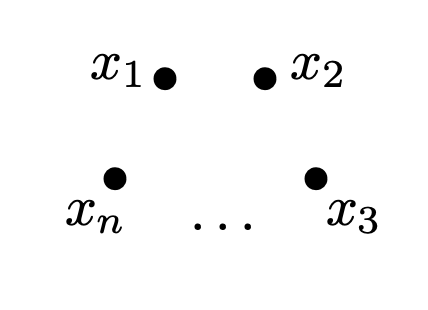
\includegraphics[scale=0.4]{fig/2.png}
\caption{Empty Graph}
\end{figure}
\end{defn}

\begin{defn}[Complete Graph]
A \textbf{complete graph}, $K_n$, is a graph $G = (V, E)$ where $V = \{x_1, \dots, x_n\}$ and $E = V^{(2)}$. Thus, $\lvert G \rvert = n$ and $\displaystyle e(G)= \binom{n}{2}$.

\begin{figure}[H]
\centering
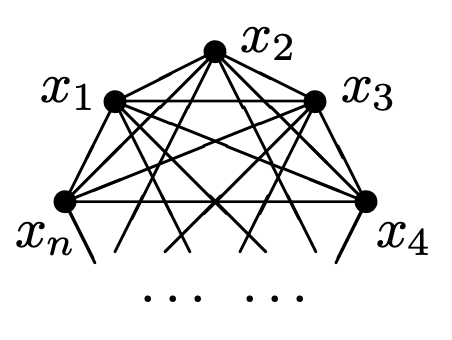
\includegraphics[scale=0.4]{fig/3.png}
\caption{Complete Graph}
\end{figure}
\end{defn}

\begin{defn}[Path]
A \textbf{path}, $P_n$, of length $n$ is a graph $G = (V, E)$ where $V = \{x_1, \dots, x_{n + 1}\}$ and $E = \{x_i x_{i + 1} : 1 \leq i \leq n\}$. Thus, $\lvert G \rvert = n + 1$ and $e(G)= n$.

\begin{figure}[H]
\centering
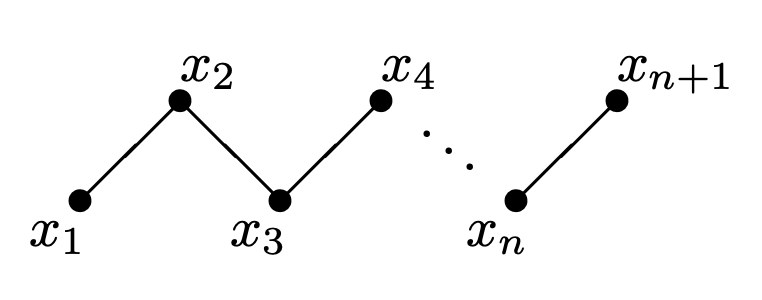
\includegraphics[scale=0.4]{fig/4.png}
\caption{Path}
\end{figure}
\end{defn}

\begin{defn}[Cycle]
A \textbf{cycle}, $C_n$, of length $n$ is a graph $G = (V, E)$ where $V = \{x_1, \dots, x_n\}$ and $E = \{x_i x_{i + 1} : 1 \leq i \leq n - 1\} \cup \{x_n x_1\}$. Thus, $\lvert G \rvert = n$ and $e(G)= n$.

\begin{figure}[H]
\centering
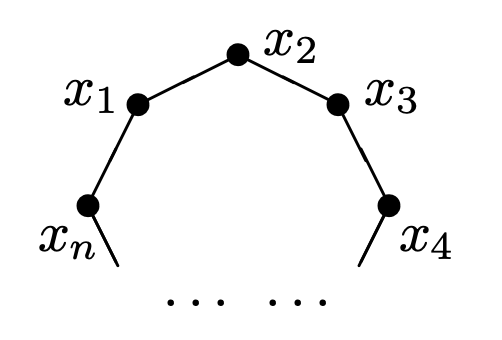
\includegraphics[scale=0.4]{fig/5.png}
\caption{Cycle}
\end{figure}
\end{defn}

\begin{defn}[Connectivity]
In an undirected graph $G$, two vertices $x$ and $y$ are called \textbf{connected} if $G$ contains a \emph{path} from $x$ to $y$. Otherwise, they are called \textbf{disconnected}.

A graph is said to be \textbf{connected} if every pair of vertices in the graph is connected. This means that there is a path between every pair of vertices.
\end{defn}

\begin{defn}[Graph Isomorphism]
Graphs $G = (V, E)$ and $H = (V', E')$ are \textbf{isomorphic} if there is a bijection $f : V \to V'$ such that $xy \in E$ if and only if $f(x)f(y) \in E'$.
\end{defn}

\begin{defn}[Subgraph]
We say that $H = (V', E')$ is a subgraph of $G = (V, E)$ if $V' \subset V$ and $E' \subset E$.
\end{defn}

\begin{rmk}
$C_n$ is a subgraph of $K_n$.
\end{rmk}

\begin{defn}[Neighborhood]
The \textbf{neighborhood} of $x$ is $\Gamma(x) = \{ y \in V : xy \in E \}$ and the \textbf{degree} of $x$ is $d(x) = \lvert \Gamma(x) \rvert$.

\begin{figure}[H]
\centering
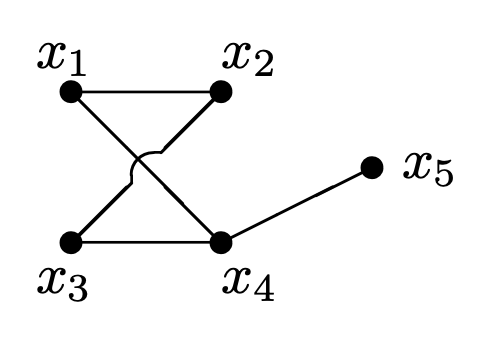
\includegraphics[scale=0.4]{fig/1.png}
\caption{$\Gamma(x_4) = \{x_1, x_3, x_5\}$, $d(x_4) = 3$.}
\end{figure}
\end{defn}

\begin{defn}[Digraph]
A \textbf{directed graph}, or \textbf{digraph}, consists of a set $V$ of \emph{vertices} (or \emph{nodes}) together with a set $E$ of ordered pairs of elements of $V$ called \emph{edges} (or \emph{arcs}). The vertex $a$ is called the \textbf{initial vertex} of the edge $(a, b)$, and the vertex $b$ is called the \textbf{terminal vertex} of this edge.

In an \textbf{undirected graph} the edges are bidirectional, with no direction associated with them. Hence, the graph can be traversed in either direction.

\begin{figure}[H]
\centering
\begin{minipage}{.5\textwidth}
  \centering
  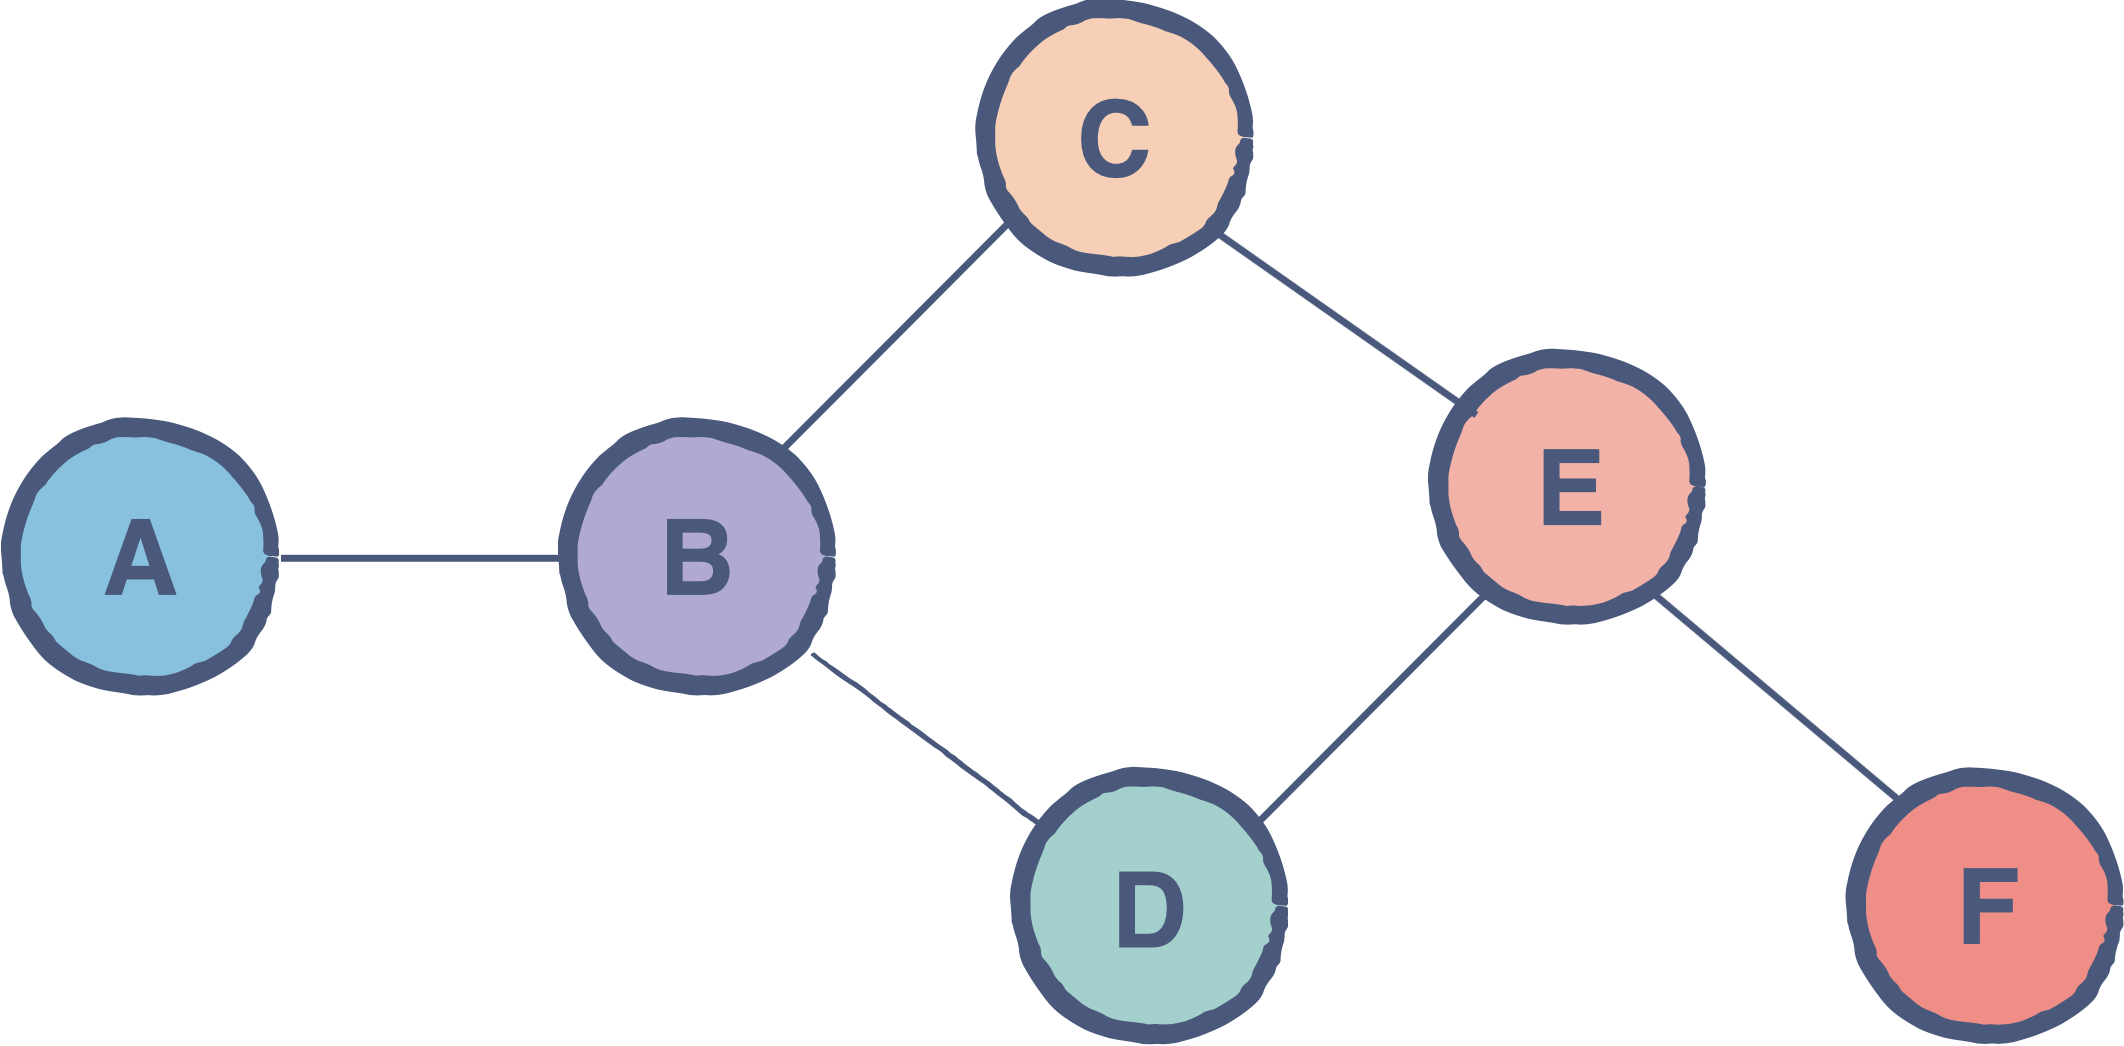
\includegraphics[scale=0.15]{fig/6.png}
  \caption{Undirected Graph}
\end{minipage}%
\begin{minipage}{.5\textwidth}
  \centering
  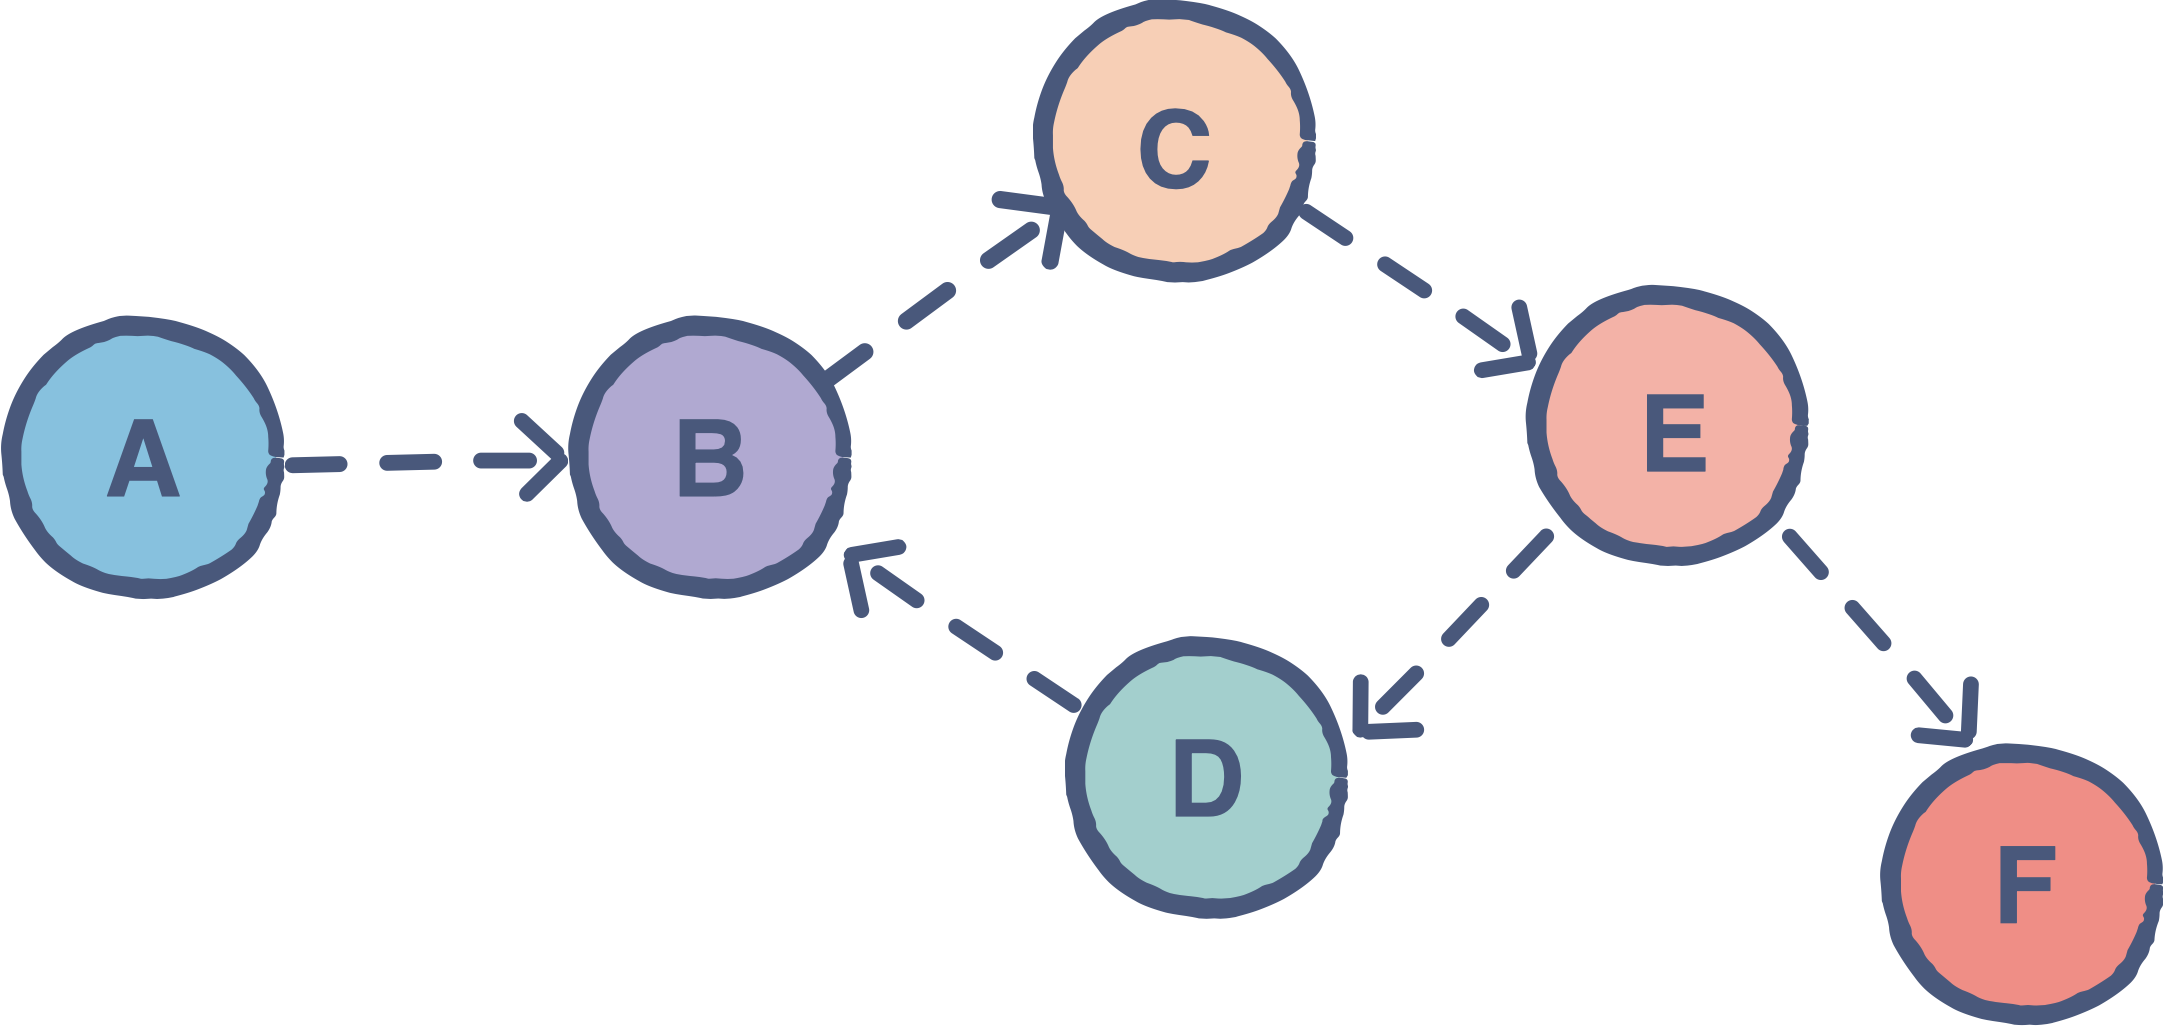
\includegraphics[scale=0.15]{fig/7.png}
  \caption{Directed Graph}
\end{minipage}
\end{figure}
\end{defn}

\hypertarget{layout}{%
\subsection{Layout}\label{layout}}

We consider economies consisting of a set
\([\ell] := \{1, \dots, \ell\}\) of \textbf{divisible goods} and a set
\([m] := \{1, \dots, m\}\) of \textbf{agents} embedded as nodes in some
graph \(G = ([m], E)\), whose edges \(E\) describe who may trade with
whom.

\begin{rmk}
For ease of exposition, $G$ is assumed undirected; all results can be easily extended to directed graphs.
\end{rmk}

In lieu of \(E\), the reflexive symmetric binary relation \(\simeq\) can
be used on \([m]\), so that for any two agents \(i, j \in [m]\), the
presence of an edge between them is denoted by \(i \simeq j\).

\begin{rmk}
For any $i, j \in [m]$, $i \sim j$ when $i \simeq j$ and $i \neq j$.
\end{rmk}

In the economy, each agent \(i \in [m]\) has an endowment of goods
\(\mathbf{e}^i \in \mathbb{R}^\ell_+\) and a utility function
\(u_i : \mathbb{R}^\ell_+ \to \mathbb{R}_+\).

\begin{defn}[Graphical Economy]
A \textbf{graphical economy} is an undirected graph $G$ over agents $[m]$ with neighbor relation $\simeq$, utilities $\{u_i : \mathbb{R}^\ell_+ \to \mathbb{R}_+\}_{i \in [m]}$, and endowments $\{\mathbf{e}^i \in \mathbb{R}^\ell_+\}_{i \in [m]}$, where $\ell$ is an integer denoting the number of goods being traded.
\end{defn}

To discuss equilibria in a graphical economy, we also need:

\begin{itemize}
\tightlist
\item
  local price vectors \(\mathbf{p}^i \in \mathbb{R}^\ell_+\) for each
  agent \(i \in [m]\), and
\item
  the bundle of goods \(\mathbf{x}^{ij} \in \mathbb{R}^\ell_+\) agent
  \(i\) purchases from agent \(j\) for consumption.
\end{itemize}

\begin{quote}
To enforce the condition that trade must traverse edges,
\(\mathbf{x}^{ij} = 0\) for \(j \not\simeq i\).
\end{quote}

\hypertarget{the-arrowdebreu-exchange-model}{%
\subsection{The Arrow--Debreu Exchange
Model}\label{the-arrowdebreu-exchange-model}}

The \citet{AD} (AD) exchange economy, also known as the Walrasian model,
is extremely well studied due to its central role in general equilibrium
theory. The graphical economies are generalizations of AD which retain
AD as a special case.

\begin{defn}[AD Equilibrium]
An \textbf{AD Equilibrium} is a pair $(\mathbf{p}, \mathbf{x})$ of a set of price vectors $\mathbf{p}$ and set of consumption plans $\mathbf{x}$ such that, if the underlying graph is complete, we have $\mathbf{p}^i = \mathbf{p}^j$ for all $i, j \in [m]$, and the following conditions are satisfied:
\end{defn}

\begin{itemize}
\tightlist
\item
  \emph{Market Clearing.}
\end{itemize}

\[
\sum_{i,j \in [m]} \mathbf{x}^{ij} = \sum_{i \in [m]} \mathbf{e}^i
\]

\begin{itemize}
\tightlist
\item
  \emph{Individual Rationality.} For all agents \(i \in [m]\), setting
  \(\hat{\mathbf{x}}^i = \mathbf{x}^i\) maximizes their utility
  \(\displaystyle u_i \left( \sum_{j \simeq i} \hat{\mathbf{x}}^{ij} \right)\)
  over all \(\hat{\mathbf{x}}^i \in \mathbb{R}^\ell_+\) satisfying
\end{itemize}

\[
\sum_{j \simeq i} \mathbf{p}^j \cdot \hat{\mathbf{x}}^{ij} \leq \mathbf{p}^i \cdot \mathbf{e}^i
\]

\hypertarget{the-kakade-kearns-ortiz-exchange-model}{%
\subsection{The Kakade, Kearns, Ortiz Exchange
Model}\label{the-kakade-kearns-ortiz-exchange-model}}

By moving from the complete graph to general graphs, and imposing a
local clearing condition instead of a global one, we arrive at the
notion of equilibria for graphical economies introduced by \citet{KKO}.

\begin{defn}[KKO Equilibrium]
A \textbf{KKO Equilibrium} is a pair $(\mathbf{p}, \mathbf{x})$ of prices $\mathbf{p} \in \mathbb{R}^{m \times \ell}$ and consumption plans $\mathbf{x} \in \mathbb{R}^{m \times m \times \ell}$ such that the following conditions are satisfied for all $i \in [m]$:
\end{defn}

\begin{itemize}
\tightlist
\item
  \emph{Local Clearing.}
\end{itemize}

\[
\sum_{j \simeq i} \mathbf{x}^{ji} = \mathbf{e}^i
\]

\begin{itemize}
\tightlist
\item
  \emph{Individual Rationality.} Setting
  \(\hat{\mathbf{x}}^i = \mathbf{x}^i\) maximizes their utility
  \(\displaystyle u_i \left( \sum_{j \simeq i} \hat{\mathbf{x}}^{ij} \right)\)
  over all \(\hat{\mathbf{x}}^i \in \mathbb{R}^{m \times \ell}_+\)
  satisfying
\end{itemize}

\[
\sum_{j \simeq i} \mathbf{p}^j \cdot \hat{\mathbf{x}}^{ij} \leq \mathbf{p}^i \cdot \mathbf{e}^i
\]

Unlike the AD equilibrium, the KKO model allows asymmetries in trade
opportunities to arise from the underlying graph, yielding local price
vectors that are generally distinct among agents.

\hypertarget{graphical-equilibrium-existence}{%
\subsection{Graphical Equilibrium
Existence}\label{graphical-equilibrium-existence}}

We begin with the assumption on utilities.

\begin{axiom}
\label{A1}
For all consumers $i$, the utility function $u_i$ satisfies the following three properties:
\end{axiom}

\begin{itemize}
\tightlist
\item
  continuity
\item
  strict monotonicity
\item
  quasi-concavity
\end{itemize}

The following facts arise from A\ref{A1} and the consumers' rationality:

\begin{enumerate}
\def\labelenumi{\arabic{enumi}.}
\tightlist
\item
  At equilibrium, the budget constraint inequality for consumer \(i\) is
  saturated, e.g.,in a standard AD economy, a consumer using an
  equilibrium plan \(\mathbf{x}^i\) spends all the money obtained from
  the sale of the endowment \(\mathbf{e}^i\).
\item
  In any graphical equilibrium, a consumer only purchases a commodity at
  the cheapest price among the neighboring consumers. Note that the
  neighboring consumer with the cheapest price may not be unique.
\end{enumerate}

\begin{axiom}[Non-Zero Endowments]
\label{A2}
For each consumer $i$ and good $k$, $e^i_k > 0$.
\end{axiom}

Essentially, A\ref{A2} in the AD setting implies that each consumer owns
a positive amount of every good in the economy. In the graphical
setting, there are effectively \(m \times \ell\) goods, but each
consumer only has an endowment in \(\ell\) of them.

\begin{defn}[Graphical Quasi-Equilibrium]
An \textbf{graphical quasi-equilibrium} is a set of globally normalized prices (i.e., $\displaystyle \sum_{i, k} p^i_k = 1$) and a set of consumption plans in which the local markets clear for each consumer $i$, with wealth $\mathbf{w}^i = \mathbf{p}^i \cdot \mathbf{e}^i$, the following condition holds:
\end{defn}

\begin{itemize}
\tightlist
\item
  \emph{Individual Rationality.} If consumer \(i\) has positive wealth,
  then \(i\) is utility-maximizing.
\item
  \emph{Individual Quasi-Rationality.} If \(i\) has no wealth, then the
  plan \(\mathbf{x}^i\) is budget constrained (and does not necessarily
  maximize utility).
\end{itemize}

\begin{lem}[Graphical Quasi-Equilibria Existence]
In any graphical economy in which A\ref{A1} holds, there exists a graphical quasi-equilibrium.
\end{lem}

\begin{lem}
If the graph of a graphical economy is connected and if A\ref{A1} and A\ref{A2} hold, then for any quasi-equilibrium set of prices $\{\mathbf{p}^i\}$, it holds that every consumer has non-zero wealth.
\end{lem}

\begin{thm}[Graphical Equilibria Existence]
For any graphical economy in which A\ref{A1} and A\ref{A2} hold, there exists a graphical equilibrium.
\end{thm}

Proof of these statements can be found in \citet{KKO}.

\hypertarget{discussion}{%
\section{Discussion}\label{discussion}}

\begin{quote}
``The graphical economics model suggests a local notion of clearance,
directly derived from that of the \citet{AD} model. Rather than asking
that the entire (global) market clear in each good, we can ask for the
stronger `provincial' conditions that the local market for each good
must clear. For instance, the United States is less concerned that the
worldwide production of beef balances worldwide demand than it is that
the production of American beef balances worldwide demand for American
beef. If this latter condition holds, the American beef industry is
doing a good job at matching the global demand for their product, even
if other countries suffer excess supply or demand.'' --- \citet{KKO}
\end{quote}

\hypertarget{relevance-to-the-economic-literature}{%
\subsection{Relevance to the Economic
Literature}\label{relevance-to-the-economic-literature}}

\begin{quote}
``Graphical games were introduced in \citet{Kearns}, where a
representation consisting of an undirected graph and a set of local
payoff matrices was proposed for multi-player games. {[}\(\dots\){]}
These provide an exponentially more succinct representation in cases
where the number of players is large, but the degree of the interaction
graph is relatively small.'' --- \citet{KKO}
\end{quote}

This first approach led to a series of papers by several authors that
established the computational benefits of this model which approximates
Nash equilibria in graphical games with a tree topology.

Inspired by this game--theoretic background, and in the same spirit,
\citet{KKO} introduce their model where one of their motivations is to
capture the fact that price differences for identical goods can arise
due to the network structure of economic interaction. The KKO model
allows for \emph{local} markets, where intuitively each agent can set
its own prices, and can purchase goods from neighboring agents at their
prices.

In order to address concerns about the centralized nature of traditional
economic models, several recent works have introduced models of
\emph{decentralized} markets. \citet{KKO} introduced a generalization of
the AD exchange model to a graphical setting, enabling a robust set of
interactions between agents on an arbitrary set of goods which is
lacking in other economic models on networks. Unfortunately, the KKO
model is ``too local'' and does not allow for any degree of
intermediation between agents.

\hypertarget{future-directions}{%
\subsection{Future Directions}\label{future-directions}}

In general, this model can allow resale, as shown in \citet{resale}, and
even graphical production settings. For instance, a node can extract
rent solely from their position in the network---strongly related to
degree centrality in graph theory.

Furthermore, in recent applied behavioral economics, these settings have
been firmly adopted in studies of wisdom convergence---that seek to
prevent the spread of misinformation to the masses---as it is in
\citet{degroot}, \citet{learn}, and, more recently, \citet{naive}.

\newpage

\bibliography{ref.bib}


\end{document}
